% -----------------------------------------------------------------------------
% Resultados
% -----------------------------------------------------------------------------

\chapter{Avaliação de Resultados}
\label{chap:resultados}

O presente capítulo é destinado à discussão dos resultados obtidos durante o desenvolvimento deste trabalho. A discussão é dividida em 2 momentos: resultados das entrevistas com \textit{stakeholders} e resultados do protótipo de biblioteca de componentes.

\section{Entrevistas com \textit{stakeholders}}
\label{sec:resEntrevistas}

No capítulo 5 deste trabalho, foi apresentada detalhadamente uma visão consolidada da percepção técnica de designers e desenvolvedores \textit{frontend} em relação à plataforma da empresa avaliada no experimento. Muitas das dores e frustrações compartilhadas por empresas que adotaram a metodologia do \textit{design system} como meio de transformação dos processos de design do seu produto, e que foram apresentadas no capítulo 3, também puderam ser percebidas pelos entrevistados.

Tomando como base as experiências compartilhadas pelos entrevistados e o \autoref{table:uxMaturity}, entende-se que a empresa avaliada encontra-se no terceiro estágio de maturidade em experiência do usuário: Embrionária. Tal classificação é justificada pelo fato de que, apesar de já existirem profissionais especializados que se preocupam com a experiência do usuário, atividades de planejamento e metrificação de valores de UX ainda não acontecem com consistência. Também não existe nenhum profissional focado em definir e disseminar diretrizes de design e UX a nível organizacional. Dessa forma, fica evidente que ainda existe um longo caminho a ser percorrido pela organização no que se diz respeito à evolução de sua maturidade de UX, e para que isso ocorra, o comprometimento de toda a organização tem vital importância.

Como forma de se medir quantitativamente o nível de satisfação dos entrevistados para com o produto da empresa, foi realizada uma simples pesquisa com os envolvidos. A pesquisa, apresentada no Anexo \ref{chap:anexoC} deste projeto, indagava, em uma escala de 1 a 10, qual o nível de satisfação do entrevistado em relação a 3 aspectos chave do produto da empresa: capacidade de escalabilidade, capacidade de reusabilidade e velocidade de desenvolvimento. A \autoref{fig:productMetrics} apresenta os resultados obtidos pela pesquisa.

\begin{figure}
  \begin{center}
	  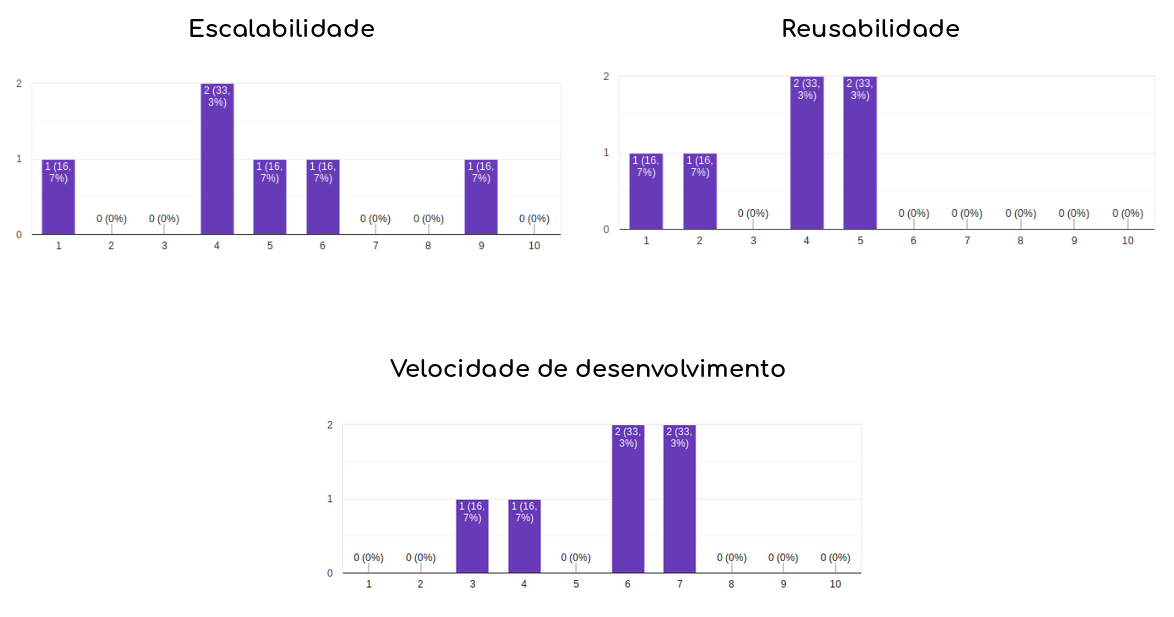
\includegraphics[width=\linewidth]{./04-figuras/08_avaliacao_resultados/product-metrics.png}
	\end{center}
  \caption{Nível de satisfação da arquitetura do produto da Dito}
  \fonte{Próprio autor}
  \label{fig:productMetrics}
\end{figure}

Para traduzir os resultados da pesquisa em um número único que reflita a atual realidade da arquitetura do produto da empresa, foi utilizada a metodologia do NPS. Em termos gerais, o \textit{Net Promoter Score} (NPS) trata-se de uma pesquisa de satisfação criada em 2003 por Fred Reichheld que, por ser simples e de fácil aplicação, acabou sendo adotada por muitas empresas, tornando-se um método universal de avaliação da satisfação de clientes \cite{nps}. Para a metodologia, as respostas da pesquisa são classificadas em 3 grupos:

\begin{itemize}
  \item Promotores: Nota 9 ou 10
  \item Neutros: Nota 7 ou 8
  \item Detratores: Notas de 1 a 6
\end{itemize}

Para o calculo do NPS, utiliza-se a seguinte fórmula:
\begin{center}
  \textbf{(Promotores - Detratores) / total de respondentes}.    
\end{center}{}

A metodologia ainda classifica os possíveis resultados do cálculo do NPS em 4 grupos:

\begin{itemize}
  \item Zona de excelência: 75\% -- 100\%
  \item Zona de qualidade: 50\% -- 74\%
  \item Zona de aperfeiçoamento: 0\% -- 49\%
  \item Zona crítica: -100\% -- -1\%
\end{itemize}

A \autoref{table:productNPS} apresenta o cálculo do NPS para as 3 diretrizes consultadas. A partir dela, conclui-se que a arquitetura do produto da empresa encontra-se em uma zona crítica, implicando que medidas devem ser tomadas o quanto antes para que a atual realidade seja revertida.

\begin{table}
  \centering
  \begin{tabular}{|m{6cm}|m{2cm}|} \hline
    
    \multicolumn{1}{|c|}{\bfseries Diretriz} & \multicolumn{1}{c|}{\bfseries NPS} \\\hline
    
    Escalabilidade & -66,67\% \\\hline
    Reusabilidade & -100\% \\\hline
    Velocidade de desenvolvimento & -66,67\% \\\hline
      
  \end{tabular}
  \caption{NPS da arquitetura do produto da Dito}
  \fonte{Próprio autor}
  \label{table:productNPS}
\end{table}


\section{Protótipo da biblioteca de componentes}

Para avaliar o valor do protótipo de biblioteca de componentes desenvolvido, foram levantadas 2 métricas base para a análise: nível de consistência das interfaces e quantidade de linhas de código-fonte. As subseções a seguir detalham cada uma das métricas, levando em consideração o atual cenário do produto da Dito e o protótipo implementado.

\subsection{Consistência nas interfaces de usuário}

Para medir a consistência em interfaces de usuário, foi realizada uma contagem do número de cores, cores de fundo, famílias de fonte e tamanhos de fonte distintos presentes nos dois objetos de estudo. A \autoref{table:interfaceConsistence}, consolida tais números.

\begin{table}
  \centering
  \begin{tabular}{|m{3cm}|m{1cm}|m{1cm}|m{1cm}|m{1cm}|} \hline
    
    \multicolumn{1}{|c|}{\bfseries Sistema} & \multicolumn{1}{c|}{\bfseries Cores} & \multicolumn{1}{c|}{\bfseries Cores de fundo} & \multicolumn{1}{c|}{\bfseries Famílias de fonte} & \multicolumn{1}{c|}{\bfseries Tamanhos de fonte} \\\hline
    
    Principal produto da Dito & 63 & 88 & 4 & 41 \\\hline
    \textit{Dito Feras} & 12 & 7 & 1 & 7 \\\hline
      
  \end{tabular}
  \caption{Consistência de interfaces de usuário}
  \fonte{Próprio autor}
  \label{table:interfaceConsistence}
\end{table}

Obviamente, comparar friamente os números dos dois sistemas não seria adequado, uma vez que o produto da empresa avaliada é muito maior e mais complexo do que o protótipo construído por este trabalho. Entretanto, contanto que a biblioteca de componentes continue evoluindo de maneira saudável, espera-se que as inconsistências evidenciadas no principal produto da Dito não se manifestem em sistemas construídos a partir de tal biblioteca.

\subsection{Quantidade de linhas de código-fonte}

Para medir fatores como velocidade de desenvolvimento, capacidade de reusabilidade e capacidade de escalabilidade, optou-se por utilizar a métrica de quantidade de linhas de código-fonte necessárias para a implementação de uma dada funcionalidade. Nesse contexto, a \autoref{table:lineCountDitoFeras} apresenta a quantidade de linhas de código-fonte utilizadas para construir artefatos do sistema \textit{DitoFeras}, já a \autoref{table:lineCountDito} faz a mesma análise levando em consideração 4 interfaces de usuários recentemente implementadas no produto da Dito.

\begin{table}
\centering
\begin{tabular}{|m{10cm}|m{1cm}|m{1cm}|m{1cm}|m{1cm}|} \hline
	
	\multicolumn{1}{|c|}{\bfseries Artefato} & \multicolumn{1}{c|}{\bfseries HTML} & \multicolumn{1}{c|}{\bfseries CSS} & \multicolumn{1}{c|}{\bfseries Javascript} \\\hline
	
	 Componente \textit{dito-box} & 0 & 9 & 10 \\\hline
	 Componente \textit{dito-color-pallet} & 0 & 20 & 0 \\\hline
	 Componente \textit{dito-text} & 0 & 64 & 0 \\\hline
	 
	 Componente \textit{dito-button} & 11 & 188 & 29 \\\hline
	 Componente \textit{dito-color-pallet-item} & 9 & 21 & 14 \\\hline
	 Componente \textit{dito-input} & 19 & 98 & 102 \\\hline
	 Componente \textit{dito-presentation-container} & 4 & 21 & 15 \\\hline
	 
	 Componente \textit{dito-form} & 0 & 0 & 34 \\\hline
	 
	 Tela de \textit{login} & 29 & 31 & 16 \\\hline
	 Tela de apresentação do componente \textit{dito-color-pallet} & 14 & 9 & 20 \\\hline
	 Tela de apresentação do componente \textit{dito-text} & 10 & 0 & 0 \\\hline
	 Tela de apresentação do componente \textit{dito-button} & 29 & 9 & 10 \\\hline
	 Tela de apresentação do componente \textit{dito-input} & 48 & 9 & 22 \\\hline
	 Tela de apresentação do componente \textit{dito-form} & 25 & 11 & 0 \\\hline
    
\end{tabular}
\caption{Quantidade de linhas de código-fonte por artefato do projeto \textit{DitoFeras}}
\fonte{Próprio autor}
\label{table:lineCountDitoFeras}
\end{table}


\begin{table}
\centering
\begin{tabular}{|m{3cm}|m{1cm}|m{1cm}|m{1cm}|m{1cm}|} \hline
	
	\multicolumn{1}{|c|}{\bfseries Artefato} & \multicolumn{1}{c|}{\bfseries HTML} & \multicolumn{1}{c|}{\bfseries CSS} & \multicolumn{1}{c|}{\bfseries Javascript} \\\hline
	 Tela 1 & 467 & 1046 & 203 \\\hline
	 Tela 2 & 98 & 257 & 258 \\\hline
	 Tela 3 & 348 & 603 & 398  \\\hline
	 Tela 4 & 837 & 1199 & 608 \\\hline
    
\end{tabular}
\caption{Quantidade de linhas de código-fonte por artefato do produto da Dito}
\fonte{Próprio autor}
\label{table:lineCountDito}
\end{table}

Guardadas as devidas proporções, percebe-se que o esforço para se construir interfaces de usuários baseadas em componentes previamente implementados é consideravelmente mais baixo. Existe um esforço inicial para se construir os componentes base das páginas, porém, uma vez implementados, o desenvolvimento de novas interfaces de usuário demonstra-se ser uma tarefa relativamente simples.

É importante mencionar, porém, que apesar de haver bastante duplicidade de código entre as soluções, as 4 interfaces selecionadas do produto da Dito para o comparativo são consideravelmente mais complexas do aquelas produzidas no protótipo. Por esse motivo, a comparação entre os números dos dois sistemas não deve acontecer de maneira literal.

Dada a simplicidade percebida no desenvolvimento de páginas baseadas em componentes, entendeu-se que o protótipo construído cumpriu o seu propósito. O valor de uma biblioteca de componentes, que no futuro poderia ser evoluída para um \textit{design system} completo e robusto, foi entendido pelos \textit{stakeholders} do projeto.

Ressalta-se, entretanto, que a escolha da tecnologia utilizada para a construção do protótipo foi falha. A empresa avaliada no experimento tinha pretenções de evoluir sua arquitetura \textit{frontend}, alterando o \textit{framework} base de suas implementações. Como a biblioteca de componentes foi construida utilizando um \textit{framework} diferente, seria inviável aproveitar o trabalho realizado na construção do protótipo em uma futura biblioteca de componentes oficial da organização.

Sabe-se que o ecossistema de tecnologia está em constante evolução. Novas tecnologias surgem a cada dia e, consequentemente, as tecnologias de ponta de hoje acabarão se tornando defasadas no futuro. Nesse contexto, entendeu-se a criação de um sistema tão importante como uma biblioteca de componentes baseado em um \textit{framework} específico não é uma decisão sustentável a longo prazo. A utilização de tecnologias como \textit{Web Components} talvez seja uma decisão mais sábia, uma vez que esta é baseada em padrões universais da Web.

Como consequência do presente trabalho, foi criado um grupo de estudos na empresa avaliada no experimento. O objetivo principal do grupo é disseminar conhecimentos a respeito dos propósitos e valores de um \textit{design system}. Foi realizada, ainda, uma atividade de descontrução de um dos mais recentes produtos da empresa, com o intuito de idealizar o esqueleto de uma biblioteca de componentes que siga os princípios do \textit{atomic design}.

Finalmente, conclui-se que um \textit{design system} é uma importante ferramenta para a diminuição da complexidade social de uma organização, promovendo melhorias na comunicação entre os colaboradores desde os momentos iniciais de sua implementação. Além disso, também se provou fundamental para a alavancagem da capacidade de escalabilidade, reusabilidade e velocidade de desenvolvimento de produtos baseados em software.
